\chapter{Apresentação do Modelo}
\label{modelo}

Conforme explicado na Seção \ref{fundamentacao:redes:construcao}, a construção de uma RB pode ser dividada em duas fases: a construção do GAD, e a definição das funções de probabilidade. Portanto, neste capítulo, serão descritas essas duas fases do processo de construção do modelo proposto neste trabalho. À princípio, será explicado como foram identificados os relacionamentos entre os fatores-chave do modelo. Em seguida, será descrito o processo adotado para a definição das funções de probabilidade, e porque foi decidido utilizar funções de probabilidade em vez de tabelas de probabilidade.

\section{Construção do GAD}
\label{modelo:gad}

Nesta fase da construção do modelo, é necessário identificar os fatores-chave que influenciam a qualidade do TE de equipes ágeis e os relacionamentos entre esses fatores. Como base para a construção do GAD, optou-se por utilizar o modelo proposto em \cite{freire} (Figura \ref{trabalho:base:modelo}). De acordo com os autores, o modelo apresentado é uma boa representação do mundo real. Entretanto, uma de suas limitações é que ele foi construído com base em apenas um trabalho. Assim, a partir desse modelo e dos fatores descritos na Seção \ref{fundamentacao:ageis:fatores}, é possível refinar o GAD, e, assim, obter uma representação mais fiel ao mundo real.

No modelo apresentado em \cite{freire}, o TE depende diretamente de três principais nós: \textit{Colaboração}, \textit{Esforço} da equipe de desenvolvimento e \textit{Atributos da Equipe}. Nesse trabalho, o fator \textit{Atributos da Equipe} depende diretamente dos \textit{Atributos Pessoais} e do \textit{Expertise} dos membros da equipe. Conforme descrito em \cite{freire}, o nó \textit{Atributos Pessoais} corresponde à diferença das personalidades dos membros da equipe, que contribui para que eles se dêem bem entre si. O nó \textit{Expertise}, por sua vez, corresponde as capacidades técnicas dos membros da equipe para realizar as atividades, com \textit{Redundância}. Assim, decidiu-se renomear o nó \textit{Atributos da Equipe} para \textit{Orientação da Equipe}, uma vez que os fatores que o influenciam afetam o respeito mútuo e a confiança existentes entre os membros da equipe. A Figura \ref{modelo:gad:orientacao} contém a representação gráfica desse nó.

\begin{figure}[ht!]
\begin{center}
		\fbox{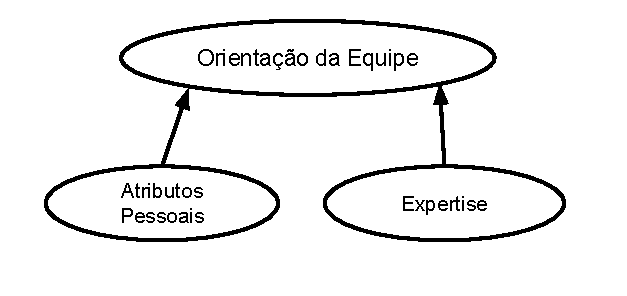
\includegraphics[scale=0.9]{figs/modeloOrientacao.pdf}}
	\end{center}
	\caption{Representação do Nó \textit{Orientação da Equipe}.}
	\label{modelo:gad:orientacao}
\end{figure}

O nó \textit{Reuniões}, que no modelo base depende diretamente dos nós \textit{Planejamento da Iteração}, \textit{Retrospectiva da Iteração} e \textit{Reuniões Diárias} foi substituído apenas pelo nó \textit{Reuniões Diárias}. Essa decisão foi tomada porque o que ocorre na \textit{Retrospectiva da Iteração}, levando em consideração a definição de \textit{Trabalho em Equipe} apresentada na Seção \ref{introducao:objetivos}, não tem influencia sobre a qualidade do TE. O \textit{Planejamento da Iteração}, por sua vez, está relacionado com a prevenção contra riscos e estimativa de tempo para cumprimento de atividades. Apesar desse fator influenciar a eficiência e o andamento da equipe, não há relação entre ele e o TE, de acordo com o que conceito definido na Seção \ref{introducao:objetivos}.

Conforme descrito em \cite{freire}, o nó \textit{Reuniões Diárias} depende diretamente dos seguintes nós: \textit{Limite de 15 Minutos}, \textit{3 Perguntas} (i.e., "O que eu fiz hoje?", "O que farei amanhã?" e "Quais obstáculos estão impedindo o meu progresso?") e \textit{Presença de Todos os Membros}. Entretanto, conforme apresentado em \cite{moe2}, \cite{gurram} e \cite{haraldsen}, o \textit{Monitoramento} é necessário para que os membros da equipe mantenham-se sincronizados em relação às atividades realizadas e problemas encontrados, além de prover \textit{Feedback} em relação à realização dessas atividades. Logo, como o objetivo das perguntas é permitir aos participantes identificar potenciais barreiras e manter a coordenação da equipe, e isso está relacionando com o \textit{Monitoramento}, decidiu-se renomear o nó \textit{3 Perguntas} para \textit{Monitoramento}. Também foi decidido remover o nó \textit{Limite de 15 minutos} porque ele não é considerado um indicador de qualidade dessas reuniões. Assim, o nó \textit{Reuniões Diárias} passou a depender apenas dos nós \textit{Monitoramento} e \textit{Presença de Todos os Membros} (Figura \ref{modelo:gad:reunioes}).

\begin{figure}[ht!]
\begin{center}
		\fbox{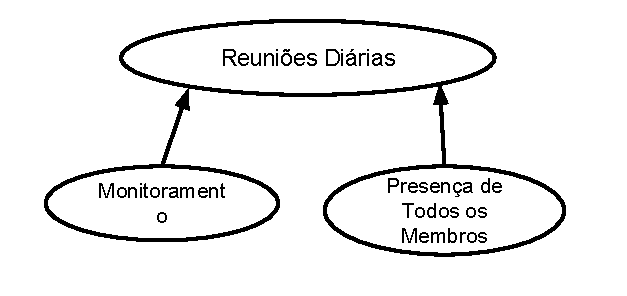
\includegraphics[scale=0.9]{figs/modeloReunioes.pdf}}
	\end{center}
	\caption{Representação do Nó \textit{Reuniões Diárias}.}
	\label{modelo:gad:reunioes}
\end{figure}

Em \cite{freire}, o nó \textit{Comunicação} depende diretamente dos seguintes nós: \textit{Frequência}, \textit{Informalidade}, \textit{Estrutura} - possibilidade dos membros da equipe se comunicarem diretamente uns com os outros - e \textit{Abertura}, que está relacionada com o ato de não haver contenção de informação entre os membros da equipe. Como forma de minimizar a complexidade dos cálculos efetuados \cite{bengal} e o viés que pode ser introduzido em virtude da subjetidade que esse nós representam, optou-se por substituir esses quatro nós por \textit{Distribuição da Equipe} e \textit{Meio de Comunicação} (Figura \ref{modelo:gad:comunicacao}), que corresponde à maneira com a qual a equipe se comunica. Esses nós estão relacionados, respectivamente, com o fato dos membros da equipe compartilharem o mesmo local de trabalho e conversarem cara-a-cara sempre que possível. Dessa forma, a \textit{Distribuição da Equipe} substitui a \textit{Frequência}, uma vez que o fato de os membros da equipe compartilharem o mesmo local facilita a comunicação \cite{lalsing} e, assim, contribui para que a comunicação ocorra em maior frequência. Já o nó \textit{Meio de Comunicação} substitui a \textit{Informalidade}, \textit{Estrutura} e \textit{Abertura}, tendo em vista que a conversa cara-a-cara contribui para que essas características se façam na presentes na \textit{Comunicação}.

\begin{figure}[ht!]
\begin{center}
		\fbox{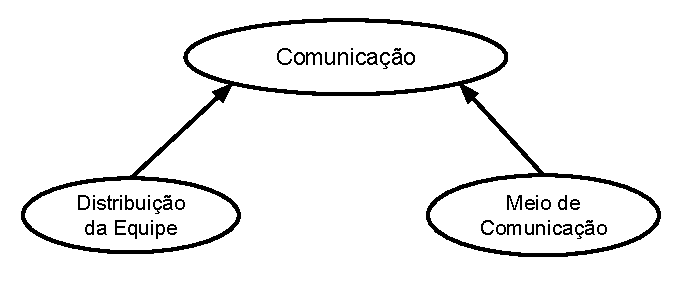
\includegraphics[scale=0.9]{figs/modeloComunicacao.pdf}}
	\end{center}
	\caption{Representação do Nó \textit{Comunicação}.}
	\label{modelo:gad:comunicacao}
\end{figure}

Na literatura, é estabelecido que a autoridade da decisão e da liderança de equipes auto-gerenciáveis precisa ser compartilhada \cite{morgan} \cite{kirkman}. Além disso, em \cite{morgan}, é dito que equipes auto-gerenciáveis requerem uma capacidade de aprendizagem das equipes para que elas possam adaptar-se às transformações que ocorrem no contexto em que o trabalho é desenvolvido. Ainda com base em \cite{morgan}, toda equipe que possui a capacidade de se auto-gerenciar precisa de um certo grau de \textit{Redundância}. Logo, com base nessas afirmações, e no fato do nó \textit{Expertise} englobar esse conceito, os nós \textit{Liderança Compartilhada}, \textit{Aprendizagem da Equipe} e \textit{Redundância} foram adicionados como pais do nó \textit{Auto-Gerenciamento}. Na Figura \ref{modelo:gad:autogerenciamento}, está representado o nó \textit{Auto-Gerenciamento}.

\begin{figure}[ht!]
\begin{center}
		\fbox{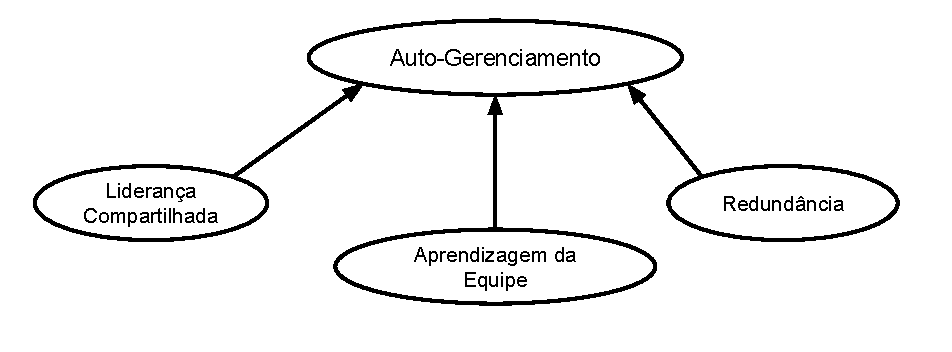
\includegraphics[scale=0.9]{figs/modeloAutoGerenciamento.pdf}}
	\end{center}
	\caption{Representação do Nó \textit{Auto-Gerenciamento}.}
	\label{modelo:gad:autogerenciamento}
\end{figure}

De acordo com a Tabela \ref{fundamentacao:ageis:fatores:tabela}, a \textit{Coordenação} de uma equipe ágil refere-se à execucação das atividades por parte dos integrantes da equipe de maneira sincronizada e integrada. Logo, com base no que foi dito anteriormente, a qualidade da \textit{Comunicação} e a eficiência das \textit{Reuniões Diárias} para sincronizar os membros da equipe com relação às atividade e problemas, contribuem para a \textit{Coordenação} da equipe.

Conforme descrito na Tabela \ref{fundamentacao:ageis:fatores:tabela}, o conceito de \textit{Colaboração} é referente ao compromisso que os integrantes tem com a equipe para alcançar os objetivos em comum. O modelo proposto em \cite{freire} considera a \textit{Comunicação} e as \textit{Reuniões} como fatores que influenciam esse nó. Contudo, neste trabalho, optou-se por considerar como pais do nó \textit{Colaboração} os seguintes nós: \textit{Coordenação} e \textit{Orientação da Equipe}. Isso porque acredita-se que eficiência da \textit{Coordenação}, e a confiança e espírito de grupo referentes aos nó \textit{Orientação da Equipe} contribuem para a \textit{Colaboração} da equipe.

O conceito de \textit{Coesão}, conforme descrito na Tabela \ref{fundamentacao:ageis:fatores:tabela}, corresponde à atração interpessoal dos membros da equipe, seu compromisso com as tarefas e espírito de grupo. Entretanto, acredita-se que, no contexto de metodologias ágeis, uma equipe coesa além de possuir essas características, que correspondem à \textit{Colaboração}. Além disso, aidan no contexto de equipes ágeis, entende-se que equipes coesas devem possuir alta capacidade de \textit{Auto-Gerenciamento}. Portanto, os nós \textit{Colaboração} e \textit{Auto-Gerenciamento} passaram a ser nós pai de \textit{Coesão}. A Figura \ref{modelo:gad:coesao} contém a representação do nó \textit{Coesão}.

\begin{figure}[ht!]
\begin{center}
		\fbox{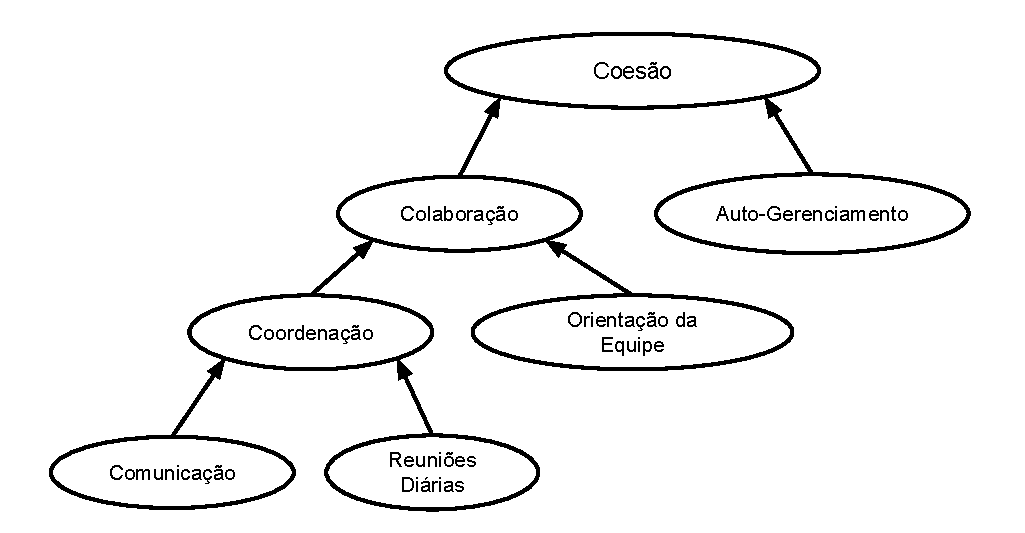
\includegraphics[scale=0.7]{figs/modeloCoesao.pdf}}
	\end{center}
	\caption{Representação do Nó \textit{Coesão}.}
	\label{modelo:gad:coesao}
\end{figure}

Na Seção \ref{introducao:objetivos}, foi definido que a interferência de um agente externo (e.g., cliente) nas atividades realizadas influencia a qualidade do TE. Essa definição é similar ao conceito do fator \textit{Autonomia da Equipe}, que refere-se à influência de agentes externos a equipe na realização das atividades dela. Portanto, foi decidido adicionar o nó \textit{Autonomia da Equipe} ao GAD. Dessa forma, considerando o conceito de \textit{Trabalho em Equipe} adotado neste trabalho, o GAD para o modelo proposto ficou definido conforme a Figura \ref{modelo:gad:final}.

\begin{figure}[ht!]
\begin{center}
		\fbox{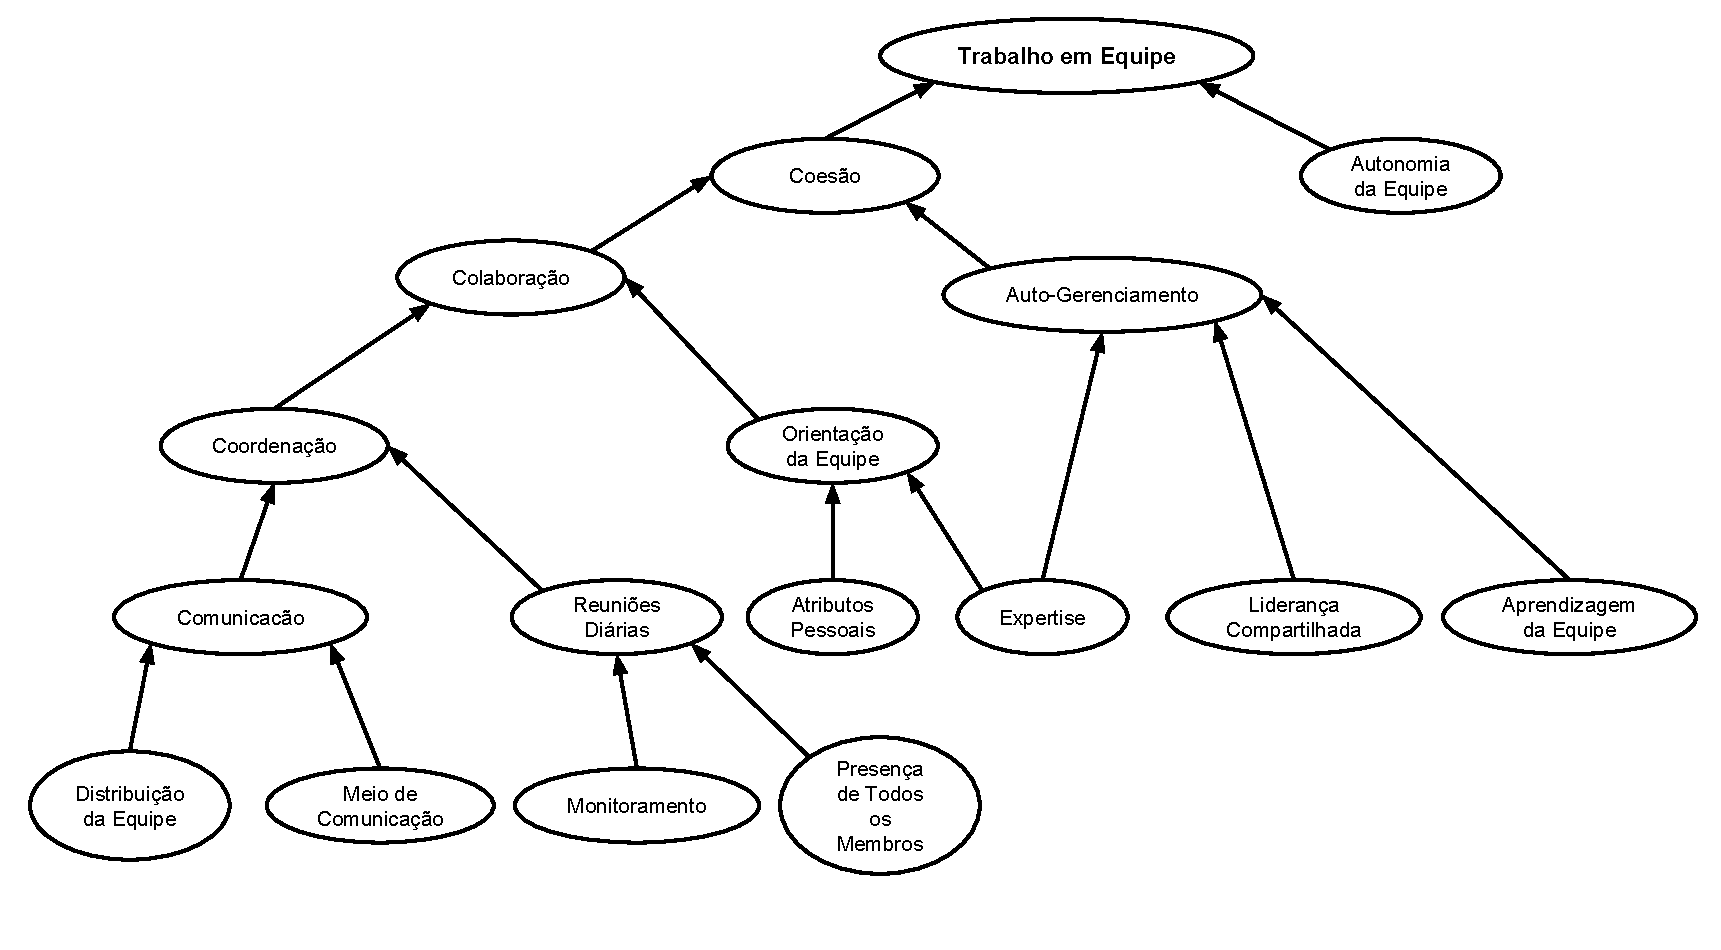
\includegraphics[scale=0.57]{figs/modeloFinal.pdf}}
	\end{center}
	\caption{Representação do Modelo Proposto.}
	\label{modelo:gad:final}
\end{figure}

Grande parte dos nós do GAD apresentados nesta seção subjetivos. Assim, como forma de minizar o viés que pode ser introduzido nos resultados calculados pelo modelo, foi decidido representar esses nós como NR, onde cada um deles possui cinco estados (i.e., Muito Baixo, Baixo, Médio, Alto e Muito Alto), onde cada estado representa um possível grau de qualidade para o nó. Portanto, os resultados calculados para cada nó, correspondem à qualidade daquele fator no cenário em que foi avaliado. Como não há evidências referentes aos nós de entrada e, de certa forma, eles também são subjetivos, também optou-se por representá-los como NR. A Tabela \ref{modelo:gad:tabela} contém as informações referentes aos significados dos estados de cada nó do modelo.

\begin{center}
\begin{longtable}{
|p{0.30\dimexpr \textwidth-3\arrayrulewidth-3\tabcolsep\relax}|
 p{0.08\dimexpr \textwidth-3\arrayrulewidth-3\tabcolsep\relax}|
 p{0.62\dimexpr \textwidth-3\arrayrulewidth-3\tabcolsep\relax}|
}
\caption{Definição dos Estados dos Nós do Modelo. \label{modelo:gad:tabela}} \\

\hline
\multicolumn{1}{|c|}{\textbf{Nó}} & \multicolumn{2}{|c|}{\textbf{Estado}} \\
\hline
\endfirsthead

\hline
\multicolumn{3}{|c|}{Continuação da Tabela \ref{satisfacao:tabela}}\\
\hline
\multicolumn{1}{|c|}{\textbf{Nó}} & \multicolumn{2}{|c|}{\textbf{Estado}} \\
\hline
\endhead

\hline
\endfoot

\hline
% \multicolumn{2}{| c |}{End of Table}\\
% \hline\hline
% \endlastfoot

\multirow{2}{*}{Trabalho em Equipe}           & Muito Alto  & Levando em consideração o conceito de TE neste trabalho, a sua qualidade é muito alta.                                                                                                \\ \cline{2-3}
                                              & Muito Baixo & Levando em consideração o conceito de TE neste trabalho, a sua qualidade é muito baixa.                                                                                               \\ \hline
\multirow{2}{*}{Autonomia da Equipe}          & Muito Alto  & Não há um agente externo interferindo em como a equipe executa suas tarefas. O agente externo colabora com a equipe para definir o que será executado e apenas quando adequado.       \\ \cline{2-3}
                                              & Muito Baixo & Há um agente externo que sempre interfere em como a equipe deve executar suas atividades.                                                                                             \\ \hline
\multirow{2}{*}{Coesão}                       & Muito Alto  & A equipe trabalha de forma coesa e síncrona, mantendo os objetivos da equipe como prioridade, com eficiência no auto-gerenciamento.                                                   \\ \cline{2-3}
                                              & Muito Baixo & A equipe não trabalha de forma coesa e síncrona, mantendo os objetivos da equipe como prioridade, sem eficiência no auto-gerenciamento.                                               \\ \hline
\multirow{2}{*}{Colaboração}                  & Muito Alto  & Há colaboração entre os membros da equipe para garantir o desenvolvimento do projeto.                                                                                                 \\ \cline{2-3}
                                              & Muito Baixo & Não há colaboração entre os membros da equipe para garantir o desenvolvimento do projeto.                                                                                             \\ \hline
\multirow{2}{*}{Auto-Gerenciamento}           & Muito Alto  & A equipe é capaz dese auto-organiza com eficácia para encarar desafios e mudanças complexas.                                                                                          \\ \cline{2-3}
                                              & Muito Baixo & A equipe não é capaz de se auto-organiza com eficácia para encarar desafios e mudanças complexas.                                                                                     \\ \hline
\multirow{2}{*}{Coordenação}                  & Muito Alto  & A execução das atividades por parte dos integrantes ocorre de maneira síncrona e integrada.                                                                                           \\ \cline{2-3}
                                              & Muito Baixo & A execução das atividades por parte dos integrantes não ocorre de maneira síncrona e integrada.                                                                                       \\ \hline
\multirow{2}{*}{Orientação da Equipe}         & Muito Alto  & Membros confiam na equipe e se sentem motivados a trabalharem juntos para alcançar os objetivos da equipe.                                                                            \\ \cline{2-3}
                                              & Muito Baixo & Membros não confiam na equipe e se sentem motivados a trabalharem juntos para alcançar os objetivos da equipe.                                                                        \\ \hline
\multirow{2}{*}{Comunicação}                  & Muito Alto  & A comunicação entre os membros da equipe é efetiva.                                                                                                                                   \\ \cline{2-3}
                                              & Muito Baixo & A comunicação entre os membros da equipe não é efetiva.                                                                                                                               \\ \hline
\multirow{2}{*}{Reuniões Diárias}             & Muito Alto  & Foi possível remover os obstáculos e sincronizar toda a equipe.                                                                                                                       \\ \cline{2-3}
                                              & Muito Baixo & Não foi possível remover os obstáculos e sincronizar toda a equipe.                                                                                                                   \\ \hline
\multirow{2}{*}{Distribuição da Equipe}       & Muito Alto  & Todos os membros da equipe compartilham o mesmo local de trabalho.                                                                                                                    \\ \cline{2-3}
                                              & Muito Baixo & Os membros da equipe compartilham o mesmo local de trabalho.                                                                                                                          \\ \hline
\multirow{2}{*}{Meio de Comunicação}          & Muito Alto  & Os membros da equipe comunicam-se cara-a-cara sempre que possível.                                                                                                                    \\ \cline{2-3}
                                              & Muito Baixo & Os membros da equipe não se comunicam cara-a-cara sempre que possível.                                                                                                                \\ \hline
\multirow{2}{*}{Monitoramento}                & Muito Alto  & Os membros da equipe externam suas dificuldades e seu progresso em relação às atividades realizadas de forma clara e objetiva.                                                        \\ \cline{2-3}
                                              & Muito Baixo & Os membros da equipe não relatam de forma clara as atividades nas quais estão envolvidos, ou aproveitam a oportunidade para justificar decisões que foram tomadas.                    \\ \hline
\multirow{2}{*}{Presença de Todos os Membros} & Muito Alto  & Todos os membros da equipe estiveram presente durante as reuniões diárias.                                                                                                            \\ \cline{2-3}
                                              & Muito Baixo & Em nenhuma das reuniões diárias todos os membros estavam presentes.                                                                                                                   \\ \hline
\multirow{2}{*}{Atributos Pessoais}           & Muito Alto  & A mistura de personalidades dos membros da equipe contribui para que eles se dêem bem entre si.                                                                                       \\ \cline{2-3}
                                              & Muito Baixo & A mistura de personalidades dos membros da equipe não contribui para que eles se dêem bem entre si.                                                                                   \\ \hline
\multirow{2}{*}{Expertise}                    & Muito Alto  & Os membros da equipe possuem todo o conhecimento necessário para o desenvolvimento das atividades com interseção (capacidade de substituir uns aos outros na realização das tarefas). \\ \cline{2-3}
                                              & Muito Baixo & Os membros da equipe NÃO possuem todo o conhecimento necessário para o desenvolvimento das atividades.                                                                                \\ \hline
\multirow{2}{*}{Liderança Compartilhada}      & Muito Alto  & A autoridade na tomada de decisões e na liderança é compartilhada entre os membros da equipe.                                                                                         \\ \cline{2-3}
                                              & Muito Baixo & A autoridade na tomada de decisões e na liderança não é compartilhada entre os membros da equipe.                                                                                     \\ \hline
\multirow{2}{*}{Aprendizagem da Equipe}       & Muito Alto  & A equipe se adapta facilmente às mudanças que ocorrem durante o projeto.                                                                                                              \\ \cline{2-3}
                                              & Muito Baixo & A equipe não tem capacidade de se adaptar às mudanças que ocorrem durante o projeto.                                                                                                  \\ \hline


\end{longtable}
\end{center} 

\section{Funções de Probabilidade}
\label{modelo:funcoes}

Levando em consideração o que foi descrito na Seção \ref{fundamentacao:redes:construcao:funcoes}, e o fato dos nós do modelo proposto neste trabalho serem NR, decidiu-se utilizar a abordagem apresentada por Laitila \cite{laitila} para definir as funções de probabilidade do modelo proposto.

Um especialista em RB e Métodos ágeis foi o responsável por definir as TPN do GAD apresentado na Seção \ref{modelo:gad}. Para cada nó filho, o especialista deve definir quais as probabilidades desse nó estar em cada estado, com base nos estados dos nós pai. Portanto, para um nó com dois pais, e tomando como exemplo a RB apresentada na Figura \ref{fundamentacao:redes:construcao:funcoes:bn1}, o especialista precisou preencher as células em branco da Tabela \ref{modelo:funcoes:tabela2nos} com as probabilidades esperadas, de forma que, para cada combinação possível $\sum_{i=1}^{n}Pi = 1$, onde $Pi$ é a probabilidade de cada estado e $n$ é a quantidade de estados possíveis do nó filho.

\begin{table}[ht!]
\centering
\caption{Tabela para Definição das Funções de Probabilidade de Nós com Dois Pais.}
\label{modelo:funcoes:tabela2nos}
\begin{tabular}{|c|c|c|c|c|c|c|}
\hline
\multicolumn{2}{|l|}{}                      & \multicolumn{5}{c|}{\textbf{Valores Esperados para Y}}                                       \\ \hline
\textbf{X1}          & \textbf{X2}          & \textbf{Muito Baixa} & \textbf{Baixa} & \textbf{Média} & \textbf{Alta} & \textbf{Muito Alta} \\ \hline
\textbf{Muito Alta}  & \textbf{Muito Baixa} &               &         &         &        &               \\ \hline
\textbf{Muito Baixa} & \textbf{Muito Alta}  &               &         &         &        &              \\ \hline
\textbf{Muito Alta}  & \textbf{Média}       &               &         &         &        &              \\ \hline
\textbf{Média}       & \textbf{Muito Alta}  &               &         &         &        &              \\ \hline
\end{tabular}
\end{table}

De maneira análoga, para cada nó filho com três pais (e.g., Figura \ref{modelo:funcoes:bn2}), porém com uma maior quantidade de combinações possíveis, o especialista precisou preencher as células em branco de uma similar à Tabela \ref{modelo:funcoes:tabela3nos}.

\begin{figure}[ht!]
\begin{center}
		\fbox{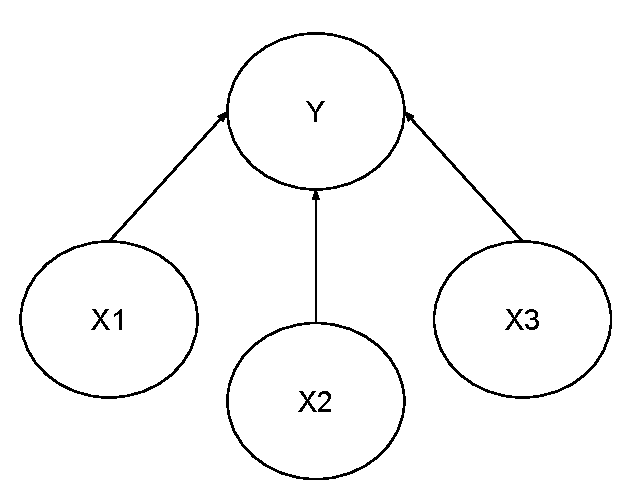
\includegraphics[scale=0.8]{figs/BN-3nos.pdf}}
	\end{center}
	\caption{Exemplo de Nó Filho com Três Pais.}
	\label{modelo:funcoes:bn2}
\end{figure}

\begin{table}[ht!]
\centering
\caption{Tabela para Definição das Funções de Probabilidade de Nós com Três Pais.}
\label{modelo:funcoes:tabela3nos}
\resizebox{\textwidth}{!}{\begin{tabular}{|c|c|c|c|c|c|c|c|}
\hline
\multicolumn{3}{|c|}{}                                             & \multicolumn{5}{c|}{\textbf{Valores Esperados para Y}}                                       \\ \hline
\textbf{X1}          & \textbf{X2}          & \textbf{X3}          & \textbf{Muito Baixa} & \textbf{Baixa} & \textbf{Média} & \textbf{Alta} & \textbf{Muito Alta} \\ \hline
\textbf{Muito Alta}  & \textbf{Muito Alta}  & \textbf{Muito Baixa} &               &         &         &        &               \\ \hline
\textbf{Muito Alta}  & \textbf{Muito Baixa} & \textbf{Muito Alta}  &               &         &         &        &               \\ \hline
\textbf{Muito Baixa} & \textbf{Muito Alta}  & \textbf{Muito Alta}  &               &         &         &        &               \\ \hline
\textbf{Muito Baixa} & \textbf{Muito Baixa} & \textbf{Muito Alta}  &               &         &         &        &               \\ \hline
\textbf{Muito Baixa} & \textbf{Muito Alta}  & \textbf{Muito Baixa} &               &         &         &        &               \\ \hline
\textbf{Muito Alta}  & \textbf{Muito Baixa} & \textbf{Muito Baixa} &               &         &         &        &               \\ \hline
\end{tabular}}
\end{table}

Assim, de acordo com a quantidade de nós pai de um determinado nó, foram definidas tabelas para cada um dos nós presentes no modelo proposto, exceto os nós de entrada. Uma vez que essas tabelas foram definidas, o especialista, com a ajuda da ferramenta AgenaRisk\footnote{\url{http://www.agenarisk.com/}}, calculou os resultados reais para cada estado. Esses cálculos foram feitos diversas vezes, pois há a necessidade de definir qual função ponderada representa a tabela de probabilidade do nó em questão, além dos pesos de cada um dos nós pai praquela função. Logo, essas repetições são necessárias até que a função e os pesos adequados, que mais se aproximem dos valores esperados, sejam encontrados. Além disso, o processo de definição das funções de probabilidade por parte do especialista é muito importante, pois caso haja inconsistências na definição do GAD, é necessário reorgarnizar a estrutura do grafo para garantir a consistência entre os conceitos e relacionamentos que estão sendo representados. Finalmente, ao final desse processo, o modelo está pronto para ser utilizado. A Tabela \ref{modelo:funcoes:tabelapesos} contém as funções e os pesos dos nós pai de todos os nós do modelo, exceto os nós de entrada.

\begin{table}[ht!]
\centering
\caption{Definição das Funções de Probabilidade.}
\label{modelo:funcoes:tabelapesos}
\resizebox{\textwidth}{!}{\begin{tabular}{|c|c|c|c|c|c|c|c|c|}
\hline
\multicolumn{3}{|c|}{\textbf{}}                                                                                                      & \multicolumn{3}{c|}{\textbf{Pais}}                                                                                                                                                                            & \multicolumn{3}{c|}{\textbf{Pesos}}                                      \\ \hline
\textbf{Nó}                                                              & \textbf{Função} & \multicolumn{1}{l|}{\textbf{Variância}} & \textbf{Pai 2}                                                    & \textbf{Pai 2}                                                         & \textbf{Pai 3}                                                   & \textbf{Peso do Pai 1} & \textbf{Peso do Pai 2} & \textbf{Peso do Pai 3} \\ \hline
\textbf{Trabalho em Equipe}                                              & WMEAN            & 0,0005                                  & Coesão                                                       & \begin{tabular}[c]{@{}c@{}}Autonomia \\ da Equipe\end{tabular}                                                    & X & 5                     & 1                     & X                     \\ \hline
\textbf{Coesão}                                                     & WMIN            & 0,0005                                  & Colaboração                                                       & Auto-Gerenciamento                                                       & X  & 3                     & 3                     & X                     \\ \hline
\textbf{Colaboração}                                                     & WMIN            & 0,0005                                  & Coordenação                                                       & \begin{tabular}[c]{@{}c@{}}Orientação \\ da Equipe\end{tabular}                                                       & X  & 5                     & 5                     & X                     \\ \hline
\textbf{Coordenação}                                                     & WMEAN            & 0,0005                                  & Comunicação                                                       & Reuniões Diárias                                                       & X  & 1                     & 1                     & X                     \\ \hline
\textbf{Comunicação}                                                     & WMIN            & 0,0005                                  & \begin{tabular}[c]{@{}c@{}}Distribuição \\ da Equipe\end{tabular} & \begin{tabular}[c]{@{}c@{}}Meio \\ de Comunicação\end{tabular}         & X                                                                & 3                      & 5                      & X                      \\ \hline
\textbf{Reuniões Diárias}                                                & WMIN            & 0,0005                                  & Monitoramento                                                     & \begin{tabular}[c]{@{}c@{}}Presença de Todos\\ os Membros\end{tabular} & X                                                                & 7                      & 7                      & X                      \\ \hline
\textbf{\begin{tabular}[c]{@{}c@{}}Orientação \\ da Equipe\end{tabular}} & WMIN            & 0,0005                                  & \begin{tabular}[c]{@{}c@{}}Atributos \\ Pessoais\end{tabular}     & Expertise                                                              & X                                                                & 5                      & 5                      & X                      \\ \hline
\textbf{Auto-Gerenciamento}                                              & WMIN            & 0,0005                                  & Expertise                                                         & \begin{tabular}[c]{@{}c@{}}Liderança \\ Compartilhada\end{tabular}     & \begin{tabular}[c]{@{}c@{}}Aprendizagem\\ da Equipe\end{tabular} & 3                      & 1                      & 1                      \\ \hline
\end{tabular}}
\end{table}
